\documentclass[conference]{IEEEtran}
% ── Font encoding (needed for accented characters: ą, ń, ż, etc.) ────────────
\usepackage[T1]{fontenc}

% ── Mathematics ───────────────────────────────────────────────────────────────
\usepackage{amsmath,amssymb,amsthm}

% ── Figures ───────────────────────────────────────────────────────────────────
\usepackage{graphicx}
\usepackage{float}
\usepackage[caption=false,font=footnotesize]{subfig}

% ── Tables ────────────────────────────────────────────────────────────────────
\usepackage{array}

% ── TikZ ──────────────────────────────────────────────────────────────────────
\usepackage{tikz}
\usetikzlibrary{shapes.geometric,arrows.meta,positioning,calc}

% ── Float control ─────────────────────────────────────────────────────────────
\usepackage{placeins}
\usepackage{stfloats}   % allows table*/figure* at bottom of two-column pages

% Relax float placement so pages fill before floats are deferred.
% Defaults (0.7/0.3/0.2/0.5) are too strict for a float-heavy two-column paper
% and cause large blocks of white space.
\renewcommand{\topfraction}{0.9}         % max page fraction for top floats
\renewcommand{\bottomfraction}{0.9}      % max page fraction for bottom floats
\renewcommand{\textfraction}{0.07}       % min page fraction that must be text
\renewcommand{\floatpagefraction}{0.75}  % min fill before a float-only page
\setcounter{topnumber}{3}
\setcounter{bottomnumber}{2}
\setcounter{totalnumber}{5}

% ── Pseudocode ────────────────────────────────────────────────────────────────
\usepackage{algorithm}
\usepackage{algpseudocode}
\algrenewcommand\algorithmicrequire{\textbf{Input:}}
\algrenewcommand\algorithmicensure{\textbf{Output:}}
\algrenewcommand\alglinenumber[1]{{\footnotesize#1}}

% ── Custom notation ───────────────────────────────────────────────────────────
\newcommand{\alphah}{\hat{\alpha}}          % estimated alpha
\newcommand{\Ph}{\hat{P}}                   % empirical PDF
\newcommand{\rhoh}{\hat{\rho}}              % estimated autocorrelation
\newcommand{\VRh}{\widehat{VR}}             % estimated variance ratio
\newcommand{\Etau}{\mathbb{E}}              % expectation

\usepackage{cite}       % BibTeX citations (\cite{})

\begin{document}

% ── Title block ───────────────────────────────────────────────────────────────
\title{Empirical L\'{e}vy Scaling in Short-Horizon Futures Returns:
       Estimation, Sensitivity, and Autocorrelation Bias}

\author{
\IEEEauthorblockN{Alexei Chekhlov}
\IEEEauthorblockA{\textit{Department of Mathematics}\\
\textit{Columbia University}\\
New York, NY, USA\\
ac3085@columbia.edu}
\and
\IEEEauthorblockN{Haoping Qiu}
\IEEEauthorblockA{\textit{Department of Statistics}\\
\textit{University of Oxford}\\
Oxford, UK\\
davinhpqiu@outlook.com}
}

% ══════════════════════════════════════════════════════════════════════════════
\maketitle

% ══════════════════════════════════════════════════════════════════════════════

% ── Abstract ──────────────────────────────────────────────────────────────────
\begin{abstract}
Short-horizon price increments in equity-index futures exhibit heavy tails
and a sharply peaked central body that is inconsistent with Gaussian dynamics,
motivating Lévy-stable distributional models.
This paper examines Lévy scaling across eight equity-index futures contracts
spanning North America and Europe, using 1-minute OHLCV data from the start
of available data through January 2026.
Three estimation approaches (peak scaling OLS, collapse quality
minimization, and fractional order structure functions) are compared
across a full factorial sensitivity analysis spanning histogram resolution,
lag grid density, and intraday seasonality correction.
All eight markets yield peak scaling exponents consistent with the
truncated Lévy-flight consensus, spanning $\alphah_{\mathrm{tip}}\in[1.718,\,1.821]$
with $R^2\geq0.997$ in every case.
The estimator choice is found to be the dominant source of variation in
reported exponents, substantially exceeding the sensitivity to tuning
parameters or intraday seasonality correction.
Finally, a closed form variance-ratio bias correction is derived for the
peak scaling estimator under short-term mean reversion and checked
cross-sectionally. The correction magnitude is found to be strongly negatively
associated with the variance ratio across markets, as the correction formula
implies.
\end{abstract}

\begin{IEEEkeywords}
Lévy-stable distributions, peak scaling estimator, equity-index futures,
variance ratio, intraday returns, self-similarity.
\end{IEEEkeywords}

% ══════════════════════════════════════════════════════════════════════════════
\section{Introduction}
\label{sec:intro}
% ══════════════════════════════════════════════════════════════════════════════

The distributional properties of short-horizon price changes have been a
central concern of financial economics and econophysics since at least
Bachelier \cite{Bachelier1900}. The Gaussian random-walk model, which predicts
normally distributed increments and variance scaling linearly with the holding
period, is a natural first approximation but a poor empirical description of
intraday returns. High-frequency data reveal distributions with heavy tails,
excess kurtosis, and a central body that is far more peaked than the Gaussian.
These features, documented across equities, foreign exchange, and derivatives
markets, motivate the use of Lévy-stable distributions as a richer
distributional model \cite{Mandelbrot1963,MantegnaStanley1994,Cont2001}.

The central prediction of the symmetric $\alpha$-stable model is
\textit{self-similarity}: the distribution of $\tau$-step price increments is
a rescaled version of the one-step distribution, with the scale factor growing
as $\tau^{1/\alpha}$ for a characteristic exponent $\alpha\in(1,2)$. This
implies that the peak of the empirical probability density
decays as $P(0,\tau)\propto\tau^{-1/\alpha}$, a relation that can be estimated
by ordinary least squares on a log-log plot and that forms the basis of the
\textit{peak scaling} approach of Mantegna and Stanley \cite{MantegnaStanley1994,MantegnaStanley1995}.
The same self-similarity predicts that empirical PDFs at different lags, when
rescaled by $\tau^{1/\alpha}$, should collapse onto a common curve, providing
a qualitative visual test of the Lévy hypothesis. Both the regression and the
collapse have been applied extensively in the econophysics literature.
Estimated exponents span a broad range of $\alpha\approx 1.5$--$1.9$ across
asset classes, frequencies, and estimation methods
\cite{Gopikrishnan1999,Weron2001,BouchaudPotters2003,Chakraborti2011}; within the narrower
setting of equity-index instruments analyzed by body or peak scaling,
estimates cluster more tightly around $\alpha\approx 1.7$--$1.8$.

Despite this activity, three important gaps remain. First, most existing
studies focus on a single market or a narrow class of instruments, typically
US equity indices or individual stocks, and it is unclear how far these results extend across different
geographies and regulatory environments. Second, the sensitivity of $\alphah$ to methodological
choices including histogram resolution, lag grid density, intraday
seasonality removal, and estimator selection has not been systematically
quantified in a single study; different choices can shift estimates by
amounts that matter for practical inference. Third, and most substantively,
the peak scaling estimator is derived under the assumption of independent
increments, yet 1-minute futures returns exhibit well-documented short-term
mean reversion driven by the bid-ask bounce and order-book dynamics
\cite{Roll1984,Bouchaud2004,ClinetPotiron2021,Yegon2025}. The direction of the resulting bias is
known qualitatively \cite{BouchaudPotters2003}, but an explicit
closed form correction and its cross-market empirical assessment
have not, to our knowledge, been jointly reported.

This paper addresses all three gaps. We use 1-minute OHLCV data for eight
equity-index futures contracts spanning North America and Europe, sourced from
TickData (Tick Data, LLC) and processed using the OneTick tick analytics
platform, covering each market from the start of available data through
January 2026. We make six contributions organized around the three gaps.

\textit{Gap 1 (cross-market coverage):}
(i)~We establish a baseline peak scaling survey across all eight markets,
reporting $\alphah_{\mathrm{tip}}$ and collapse diagnostics for each.
(v)~We test the symmetry assumption of the Lévy model by computing the
pointwise asymmetry of the empirical PDFs and examining whether symmetrization
improves collapse quality.

\textit{Gap 2 (methodological sensitivity):}
(ii)~We test the effect of intraday seasonality removal on $\alphah$, running
the full PDF analysis on both raw and deseasonalized price series and
comparing the resulting estimates.
(iii)~We compare three distinct estimators (tip scaling OLS,
collapse quality minimization, and fractional order structure functions)
across all markets to assess their mutual consistency.
(iv)~We construct a full factorial robustness matrix spanning all combinations
of histogram resolution, lag grid density, preprocessing choice, and
estimator, and decompose the variance of $\alphah$ across these factors to
identify which choices matter most.

\textit{Gap 3 (bias correction):}
(vi)~We derive a closed form bias correction for the peak scaling estimator
under short-term mean reversion, express it in terms of the
Campbell--Lo--MacKinlay variance ratio, and evaluate it across all eight
markets.

The paper is organized as follows. Section~\ref{sec:background} provides
the theoretical background on Lévy-stable distributions, peak scaling
estimation, and the variance-ratio framework. Section~\ref{sec:data} describes
the data and preprocessing steps. Section~\ref{sec:methodology} develops the
six analytical methods in detail. Section~\ref{sec:results} presents the
results for each contribution. Section~\ref{sec:conclusion} summarizes the
findings, discusses limitations, and suggests extensions.


% ══════════════════════════════════════════════════════════════════════════════
\section{Background}
\label{sec:background}
% ══════════════════════════════════════════════════════════════════════════════

\subsection{Lévy-stable distributions and the peak scaling formula}
\label{sec:background:levy}

The generalized central limit theorem establishes that the stable
distributions are the complete set of non-degenerate distributional limits of
normalized sums of i.i.d.\ random variables \cite{SamorodTaqqu1994,GnedenkoKolmogorov1954,Nolan2020}.
A symmetric $\alpha$-stable variable $X \sim S_\alpha(\gamma,0,0)$ has
characteristic function
\begin{equation}
  \Etau\!\left[e^{iqX}\right] = \exp\!\left(-\gamma|q|^\alpha\right),
  \quad \gamma > 0,\quad \alpha \in (0,2].
  \label{eq:cf}
\end{equation}
The Gaussian ($\alpha = 2$) is the unique finite-variance special case; for
$\alpha < 2$ the tails decay algebraically as $P(|X|>u)\sim C_\alpha u^{-\alpha}$,
so all moments of order $\geq\alpha$ are infinite.

For i.i.d.\ increments drawn from $S_\alpha(\gamma,0,0)$, the $\tau$-step sum
has coefficient $\gamma\tau$, yielding the self-similarity property
\begin{equation}
  P_{\alpha,\gamma}(x,\tau)
  = (\gamma\tau)^{-1/\alpha}
    F_\alpha\!\left(\frac{x}{(\gamma\tau)^{1/\alpha}}\right),
  \label{eq:scaling}
\end{equation}
where $F_\alpha$ is the standardized stable density. This scaling form is the
central prediction of the Lévy model: the shape of the increment distribution
is identical at every lag, up to a scale factor growing as $\tau^{1/\alpha}$.
Setting $x=0$ and using $F_\alpha(0) = \Gamma(1/\alpha)/(\pi\alpha)$ gives the
\textit{peak scaling formula}
\begin{equation}
  P(0,\tau)
  = \frac{\Gamma(1/\alpha)}{\pi\alpha}\,(\gamma\tau)^{-1/\alpha}.
  \label{eq:peak}
\end{equation}
The log-log regression of $\Ph(0,\tau)$ on $\tau$ therefore has slope
$-1/\alpha$, independent of the scale coefficient $\gamma$.

Mandelbrot \cite{Mandelbrot1963} first proposed that asset-price increments lie in
the domain of attraction of a stable law with $\alpha\in(1,2)$.
Mantegna and Stanley \cite{MantegnaStanley1994,MantegnaStanley1995} provided the first
systematic intraday evidence using S\&P 500 data, finding $\alpha\approx 1.40$
over three orders of magnitude in lag and demonstrating clean PDF collapse.
The truncated Lévy flight (TLF) resolves the tension between
infinite-variance stable laws and finite empirical moments: the distribution
follows the stable power law over intermediate scales but is exponentially
cut off in the far tail, producing finite variance while preserving
Lévy-like body scaling over the observable range
\cite{MantegnaStanley1994,BouchaudPotters2003}. Weron \cite{Weron2001}
showed that even samples on the order of $10^6$ can still yield seriously
upward-biased tail-index estimates when $\alpha$ is close to 2, with the
severity depending on the estimator and the tail cutoff, so empirical
$\alphah$ estimates are best interpreted as body-scaling parameters rather
than tail-index claims.

Plerou et al.\ \cite{Plerou1999} extended the analysis to individual US
companies and found power-law tails with exponent $\zeta\approx 3$, outside
the Lévy-stable regime in the strict sense, matching the index-level result
of Gopikrishnan et al.\ \cite{Gopikrishnan1999}. Weron \cite{Weron2001} showed this apparent
discrepancy is a finite-sample artifact: a Lévy-stable distribution with
$\alpha\approx 1.7$-$1.8$ produces Hill-estimator values of $\zeta\approx 3$
on samples of realistic size. This reconciliation motivates the
multi-estimator approach used here and the conservative
interpretation of $\alphah$ as a central-body parameter. More recent work by
W{\k{a}}torek et al.\ \cite{Masoliver2021} and Ratliff-Crain et al.\ \cite{ContMiami2023} confirms that the
central-body Lévy-scaling picture is stable through the 2010s, justifying its
application to contemporary futures data.

\subsection{Estimation of the scaling exponent}
\label{sec:background:estimation}

Three estimation strategies are commonly used in the literature.

The \textit{peak scaling OLS} estimator, introduced by
Mantegna and Stanley \cite{MantegnaStanley1994}, regresses $\log\Ph(0,\tau)$ on $\log\tau$ and
recovers $\alphah_{\mathrm{tip}} = -1/\hat{m}$ from the slope $\hat{m}$.
The estimator is semiparametric as it uses only the value of the distribution
at the origin and makes no assumption about the shape elsewhere.

The \textit{collapse quality} estimator, formulated here as an operational
criterion for the visual PDF-collapse test used throughout the econophysics
literature \cite{MantegnaStanley1995,Gopikrishnan1999}, chooses
$\alpha$ to minimize the spread of the rescaled empirical curves
$\tau^{1/\alpha}\Ph(\tau^{1/\alpha}\tilde{x},\tau)$ around a common function.
A mean-squared log-deviation score weights the central body and the tails
more evenly than a pure-origin regression, providing an independent route to
$\alphah$ that does not rely on a single histogram bin.

The \textit{fractional structure function} estimator
\cite{MuzyBacry1993,BouchaudPotters2003,Jiang2019,Saadaoui2024,Masoudi2025} exploits the prediction
$S_q(\tau) = \Etau[|\Delta P_\tau|^q] \propto \tau^{q/\alpha}$ for $q <
\alpha$. A log-log regression of $\hat{S}_q(\tau)$ on $\tau$ yields
slope $q/\alphah_q$; the median across moment orders
$q\in\{0.25,0.5,0.75,1.0,1.25,1.5\}$ gives $\alphah_{\mathrm{sf}}$.
Fractional orders $q\in(0,1)$ downweight outliers and converge reliably on
moderate samples \cite{Uchaikin2003}, while $q\in(1,\alpha)$ are
sensitive to the tail. Systematic concavity of the empirical scaling exponent
$\hat\zeta(q) = q/\alphah_q$ would signal multifractal corrections beyond
simple Lévy scaling \cite{Mandelbrot1997,MuzyBacry1993}.

Weron \cite{Weron2001} and Baru\v{n}\'ik and Va\v{c}ha \cite{Barunik2010}
document severe finite-sample upward bias in Hill-type tail-index estimates
when $\alpha$ is near 2, which motivates the use of body-based semiparametric
estimators such as the three adopted here in place of direct tail-index
estimation. The comparison of the three estimators across all eight
markets is central to the robustness analysis of Section~\ref{sec:results:robustness}.

These three semiparametric estimators are preferred over parametric
maximum-likelihood (MLE) approaches for three reasons.
First, the Lévy-stable density has no closed form expression for general
$\alpha\in(1,2)$, requiring numerical characteristic-function inversion at
each function evaluation. MLE is therefore computationally intensive and
numerically sensitive, particularly near $\alpha=2$ where the density
converges to the Gaussian \cite{Nolan2020}.
Second, MLE jointly estimates the full four-parameter stable vector
$(\alpha,\beta,\gamma,\delta)$, introducing estimation uncertainty in the
nuisance parameters $\beta$ (skewness) and $\delta$ (location) that
propagates into the target parameter $\alpha$. The three semiparametric
methods focus entirely on the scaling exponent, treating shape and location
as nuisances.
Third, each of the three methods targets a geometrically distinct aspect of
the self-similar scaling: the peak estimator uses the origin density at each
lag, the collapse estimator uses the full rescaled shape across all lags
simultaneously, and the structure function estimator uses moment scaling.
Agreement among three geometrically independent routes to $\alphah$
therefore constitutes stronger evidence for the Lévy hypothesis than any
single estimator, including MLE.

\subsection{Short-term dependence and the variance-ratio bias}
\label{sec:background:vr}

Lo and MacKinlay \cite{LoMacKinlay1988} introduced the variance ratio
\begin{equation}
  VR(\tau) = \frac{\mathrm{Var}(\Delta P_\tau)}{\tau\,\mathrm{Var}(\delta_1)},
  \label{eq:vr}
\end{equation}
which equals 1 under i.i.d.\ increments, exceeds 1 under positive serial
correlation, and falls below 1 under mean reversion. It remains the standard
tool for characterizing horizon-dependent memory in returns and has recently
been generalized to the multivariate cross section \cite{Froseth2026}.
The exact relationship to the autocorrelation function is
\begin{equation}
  VR(\tau)
  = 1 + 2\sum_{k=1}^{\tau-1}\!\left(1-\frac{k}{\tau}\right)\rho(k),
  \label{eq:vr_rho}
\end{equation}
which forms the basis for both variance-ratio estimators implemented here.

At 1-minute frequency the dominant effect is mean reversion, not the positive
correlation found at weekly horizons by Lo and MacKinlay \cite{LoMacKinlay1988}.
Two mechanisms contribute to this mean reversion. Roll \cite{Roll1984} showed that the bid-ask bounce
generates a spurious first-order autocovariance $\mathrm{Cov}(\Delta p_t,\Delta p_{t-1})\approx -s^2/4$ for effective spread $s$, a purely mechanical effect. Bouchaud et al.\ \cite{Bouchaud2004} and
Farmer et al.\ \cite{Farmer2006} documented that large market orders move prices but
this impact partially reverts as the order book replenishes, adding genuine
mean reversion at short horizons. Bouchaud and Potters \cite{BouchaudPotters2003} (Ch.~6)
report $\rhoh(1)\approx -0.1$ to $-0.2$ at 1-minute frequency in major
equity-index futures, consistent with the values reported here.
Recent work continues to document these effects at minute-level resolution
in a contemporary equity-index ETF \cite{Deep2025}.

The canonical peak formula~\eqref{eq:peak} is derived under strictly
independent increments. When $VR(\tau)\neq 1$, the effective Lévy scale at
lag $\tau$ is modified. The derivation proceeds in two steps.
First, by the definition of the variance ratio in Equation~\eqref{eq:vr},
the spread of $\Delta P_\tau$ under correlated increments satisfies
$\mathrm{Var}(\Delta P_\tau)=\tau\,\mathrm{Var}(\delta_1)\cdot VR(\tau)$,
i.e., the ``dispersion'' of the $\tau$-step sum is scaled by $\sqrt{VR(\tau)}$
relative to the i.i.d.\ baseline.
Second, for a symmetric $\alpha$-stable distribution the scale parameter
$\gamma$ transforms as $\gamma\mapsto c^\alpha\gamma$ under a linear scaling
$X\mapsto cX$ (homogeneity of the stable CF); hence scaling the dispersion
by $\sqrt{VR(\tau)}$ scales $\gamma$ by $(\sqrt{VR(\tau)})^\alpha
= VR(\tau)^{\alpha/2}$.
Combining, the effective Lévy scale at lag $\tau$ is
\begin{equation}
  \gamma_{\mathrm{eff}}(\tau) = \gamma\tau\cdot VR(\tau)^{\alpha/2},
  \label{eq:gamma_eff}
\end{equation}
and substituting into Equation~\eqref{eq:peak} gives the corrected
log-peak regression
\begin{equation}
  \log P(0,\tau)
  = -\frac{1}{\alpha}\log\tau
    - \frac{1}{2}\log VR(\tau)
    + \mathrm{const}.
  \label{eq:corrected_peak}
\end{equation}
The direction of the resulting slope bias
$\mathrm{Cov}(\log\tau,\,-\tfrac12\log VR(\tau))/\mathrm{Var}(\log\tau)$ is hence governed by how $VR(\tau)$ varies with the aggregation
horizon rather than by its level. Note that a constant variance ratio, regardless of distance from unity, shifts only the intercept. In the estimated profiles $VR(\tau)$
declines with $\tau$, so $-\tfrac12\log VR(\tau)$ is positively associated
with $\log\tau$. Omitting it hence makes the raw OLS slope less negative and biases
$\alphah_{\mathrm{tip}}$ upward toward the Gaussian boundary.

\textit{Remark (heuristic nature of the correction).}
The derivation above relies on the homogeneity property of the stable
characteristic function, which holds exactly for a pure $\alpha$-stable
law where the variance $\mathrm{Var}(\Delta P_\tau)$ is formally infinite.
In our empirical setting the relevant model is a truncated Lévy flight (TLF),
which has finite variance. The variance ratio $VR(\tau)$ is therefore
well defined but the stable homogeneity step is only approximate for TLF.
The correction is best understood as a heuristic: the second-order moment
variance ratio proxies for the scale distortion over the observable body of
the distribution, not a rigorous stable-law result.
The correction
procedure is developed in Section~\ref{sec:methodology:bias}. To our knowledge, the explicit OLS bias formula in the
Campbell--Lo--MacKinlay variance-ratio form and its cross-market empirical
validation have not been jointly reported; Bouchaud and Potters \cite{BouchaudPotters2003}
(Ch.~6) discuss the qualitative direction of the effect but do not derive
the specific correction term or validate it across a cross section of markets.


% ══════════════════════════════════════════════════════════════════════════════
\section{Data}
\label{sec:data}
% ══════════════════════════════════════════════════════════════════════════════

\begin{table*}[!t]
\begin{center}
\caption{Sample Futures Contracts}
\footnotesize
\begin{tabular}{lllllrrr}
\hline
Symbol & Name & Exchange & Sample Start$^{\dagger}$ & Session & Days & Records & Filled (\%) \\
\hline
YM & Dow Jones E-mini      & CBOT/CME          & May 2002 & 08:30--15:15 & 6{,}078 & 2{,}422{,}689 & 0.2 \\
NQ & NASDAQ-100 E-mini     & CME               & Jul 1999 & 08:30--15:15 & 6{,}811 & 2{,}710{,}209 & 0.2 \\
ER & Russell 2000 E-mini   & ICE Futures US    & Jan 2002 & 08:30--15:15 & 6{,}190 & 2{,}379{,}137 & 3.8 \\
ES & S\&P 500 E-mini       & CME               & Sep 1997 & 08:30--15:15 & 7{,}266 & 2{,}895{,}667 & 0.1 \\
PT & S\&P/TSX 60           & MX (Montr\'{e}al) & Oct 1999 & 09:30--16:15 & 6{,}586 & 2{,}328{,}757 & 12.5 \\
FT & FTSE 100              & ICE Futures       & Jul 1998 & 08:00--16:30 & 6{,}954 & 3{,}489{,}481 & 1.2 \\
DA & DAX                   & EUREX             & Jan 1997 & 09:00--17:30 & 7{,}370 & 3{,}721{,}908 & 0.4 \\
CF & CAC-40                & Euronext          & May 2000 & 09:00--17:30 & 6{,}578 & 3{,}328{,}132 & 0.5 \\
\hline
\multicolumn{8}{l}{$^{\dagger}$Start of available data in our sample; several contracts listed earlier (DA: Nov 1990,}\\
\multicolumn{8}{l}{\phantom{$^{\dagger}$}FT: May 1984, CF: 1988). ER: CME to 2008, ICE Futures US (then NYBOT) 2008--2017, CME from Jul 2017.}\\
\multicolumn{8}{l}{Records: observed 1-minute bars. Filled: share of the session-minute grid supplied by LOCF.}\\
\end{tabular}
\label{tab:markets}
\end{center}
\end{table*}

\subsection{Markets and sample}
\label{sec:data:markets}

The dataset consists of 1-minute resolution day-session price histories for
eight equity-index futures contracts spanning four geographical regions. The
1-minute OHLCV data were obtained from TickData (Tick Data, LLC) and processed
using the OneTick tick analytics platform, covering each market from the start
of available data through 14 January 2026. The files are supplied as
preconstructed continuous day-session series; the vendor's ``skip'' option
omits any minute with no recorded transaction, which motivates the gap-filling
step below. The contract-month selection and roll convention underlying the
continuous series are fixed by the vendor and are not exposed in the
delivered files. Table~\ref{tab:markets} provides a full description of each
contract.


The eight contracts were selected to provide a focused cross section of
liquid equity-index futures across geographies rather than on the basis of
any statistical pre-screening. Four North American equity-index contracts trade at major US venues: YM, NQ, and ES on CME Group exchanges, and ER on CME and ICE Futures US at different points in the sample (Table~\ref{tab:markets}); one Canadian contract (PT) trades on the Montr\'{e}al Exchange (MX); and three European contracts (FT, DA, CF) cover the major continental and UK equity benchmarks.

Equity-index futures are chosen over alternative liquid asset
classes such as foreign exchange (FX) and sovereign fixed income for three main
reasons.
First, equity-index futures are the canonical setting of the empirical
Lévy-scaling literature. The peak scaling approach of Mantegna and Stanley
\cite{MantegnaStanley1994,MantegnaStanley1995} was developed on S\&P~500
intraday data, and the present study is most directly interpreted as an
extension of that literature to an international cross section.
Second, equity-index futures trade on regulated, centralized exchanges with
standardized contract specifications and electronically matched price
discovery, making microstructure properties, in particular the bid-ask
bounce mechanism that motivates the bias correction in
Section~\ref{sec:background:vr}, well characterized and consistent across
venues \cite{Roll1984,Bouchaud2004,ClinetPotiron2021}. In comparison, foreign exchange
markets are predominantly over-the-counter; effective spreads and price
formation mechanisms vary substantially across dealers and platforms,
complicating systematic cross-market comparison.
Third, at 1-minute frequency the price dynamics of equity-index futures are
driven by a single dominant risk factor, namely aggregate equity market
risk, whereas fixed-income futures are governed by duration-weighted interest rate
expectations that produce materially different distributional properties at
high frequency. The extension of these results to other asset classes is an
open question noted in Section~\ref{sec:conclusion}.

The raw data files are stored in ``skip'' format: minutes with no transactions are
omitted from the file rather than recorded as zero-volume observations. This
is further addressed in preprocessing (Section~\ref{sec:data:preprocessing}).

To justify the use of 1-minute price changes as the elementary increment,
Table~\ref{tab:sigma} reports for each market the reference value of the
1-minute price change scale $\sigma_1$, the average effective bid-ask spread $s$,
and the tick size $\Delta$ (the minimum quotable price increment).
The relevant criterion concerns the \textit{bid-ask bounce}: when successive
trades arrive alternately at the bid and the ask, they generate a spurious
price change of one effective spread with no movement in the underlying price
\cite{Roll1984}. Genuine price variation must therefore dominate the bounce
amplitude which requires $\sigma_1/s > 1$; below unity, a substantial
fraction of recorded increments would reflect the bounce rather than true
price movement. The ratio exceeds 1 for all eight contracts, ranging from
$1.11$ (FT) to $4.90$ (NQ), confirming that the 1-minute frequency is
informative across the full cross section.
Note that the bounce is additionally the mechanism
generating the short-term mean reversion for which
Section~\ref{sec:background:vr} derives an explicit correction.
The tick size is reported as it sets the resolution of
the histogram grid used throughout Section~\ref{sec:methodology}, where the
bin width is defined as a multiple of $\Delta$. It is also relevant to the
scaling analysis itself. Curato and Lillo \cite{CuratoLillo2015} show that
when the tick-to-price ratio is large, price discreteness induces clustering
in the return distribution that distorts its high-frequency scaling. This
effect attenuates as the observation scale increases and therefore acts
on the lag dependence that the peak scaling estimator exploits. All eight
contracts have 1-minute volatility exceeding one tick, with $\sigma_1/\Delta$
between $2.7$ and $9.3$, which reduces but does not eliminate the possibility
that discreteness dominates the central bin. Gap-filling contributes zero
increments directly, so the atom at the origin is largest for the markets with
the highest fill rates (Table~\ref{tab:markets}).

\begin{table}[!t]
\begin{center}
\caption{Market Volatility, Tick Size and Effective Spread}
\begin{tabular}{lrrrrr}
\hline
Market & $\sigma_1$ & $\Delta$ (tick) & $\sigma_1/\Delta$ & $s$ (spread) & $\sigma_1/s$ \\
\hline
YM & 6.15 & 1.00 & 6.15 & 1.30 & 4.73 \\
NQ & 2.33 & 0.25 & 9.31 & 0.48 & 4.90 \\
ER & 0.51 & 0.10 & 5.11 & 0.22 & 2.32 \\
ES & 0.68 & 0.25 & 2.71 & 0.25 & 2.71 \\
PT & 0.46 & 0.10 & 4.59 & 0.22 & 2.09 \\
FT & 2.78 & 0.50 & 5.56 & 2.50 & 1.11 \\
DA & 3.48 & 0.50 & 6.97 & 1.20 & 2.90 \\
CF & 2.61 & 0.50 & 5.23 & 2.00 & 1.31 \\
\hline
\multicolumn{6}{l}{\small $\sigma_1$, $\Delta$ and $s$ in native contract price units (index points);}\\
\multicolumn{6}{l}{\small $s$ is the average quoted bid-ask spread. $\sigma_1$ is the reference}\\
\multicolumn{6}{l}{\small specification value used to calibrate the histogram grid; a whole-sample}\\
\multicolumn{6}{l}{\small estimate differs, since point volatility grew with index levels.}\\
\end{tabular}
\label{tab:sigma}
\end{center}
\end{table}

\subsection{Preprocessing}
\label{sec:data:preprocessing}

Three preprocessing steps are applied uniformly across all markets before any
statistical analysis.

\textit{Integer-scale conversion.} To work in integer arithmetic and avoid
floating-point accumulation errors, each price series is multiplied by a
contract-specific decimal multiplier $M$ and rounded to the nearest integer.
The multiplier is the smallest power of ten that renders the quoted prices
integral ($M=1$ for YM; $M=10$ for ER, PT, FT, DA and CF; $M=100$ for NQ and
ES), so one integer unit equals one unit in the last quoted decimal place
rather than one tick. All subsequent price differences are therefore
integers. The tick size $\Delta$ enters separately, through the
construction of the histogram grid described in
Section~\ref{sec:methodology:pdf}.

\textit{Gap-filling.} The raw files omit minutes with no transactions. Missing
minutes within a trading session are filled by carrying forward the last
observed price (last-observation-carried-forward, LOCF). This preserves the
equal spacing of the 1-minute grid required for the lag-$\tau$ increment
construction while recording zero price change during illiquid periods, which
imposes a zero recorded increment during the missing interval. Sessions are
concatenated on a continuous session-minute index, so $\tau$ throughout this
paper counts \emph{session} minutes rather than elapsed clock minutes: nights,
weekends and holidays are removed from the time axis, and each overnight price
change is compressed into a single index step. Two consequences follow. At
short lags the increment population is a mixture: a fraction $\min(\tau/J,1)$ of
$\tau$-step increments straddles an overnight boundary, rising from about
$0.2\%$ at $\tau=1$ to unity at one full session ($J=405$ or $510$ minutes), so the identically distributed assumption
underlying Equation~\eqref{eq:scaling} holds only approximately. At lags
beyond one session every increment spans at least one overnight period, which
is the intended meaning of a multi-day price change but makes the aggregation
horizon a business-time rather than a calendar-time quantity. Excluding the
shortest lags does not remove this feature, and it is retained as a limitation.

\textit{Lag grid construction.} Price increments $\delta_\tau(t) = P(t) -
P(t-\tau)$ are formed for each lag $\tau$ on two log-spaced grids. Following
the econophysics convention, ``return'' is used throughout for the price
increment $\delta_\tau$ measured in native index points; no proportional or
logarithmic transformation is applied at any stage. The coarse
grid ($N_\tau = 20$) spans $\tau \in \{1, 2, 3, 6, \ldots, 56{,}234\}$
minutes; the fine grid ($N_\tau = 37$) spans the same range with higher
density. The maximum lag of 56,234 minutes corresponds to approximately six
months of trading for a 405-minute session. Both grids are used in all
estimations to assess the sensitivity of $\alphah$ to the choice of $N_\tau$.


% ══════════════════════════════════════════════════════════════════════════════
\section{Methodology}
\label{sec:methodology}
% ══════════════════════════════════════════════════════════════════════════════

\subsection{Empirical PDF estimation}
\label{sec:methodology:pdf}

For each market and lag $\tau$ on the grid, price increments
$\Delta P_\tau(t) = P(t) - P(t-\tau)$ are formed from the gap-filled
integer-scaled price series and binned on a symmetric grid of $N_x+1 = 2{,}001$
equally spaced bin centers spanning $[-x_{\max},\,x_{\max}]$, which define
$N_x = 2{,}000$ intervals of equal width. Following the reference
implementation, the half-width is set as a tick-relative multiple of the
typical 1-minute move,
\begin{equation}
  x_{\max} = M\,\Delta\cdot N_x\cdot
             \max\!\left(\left\lfloor\varepsilon\,\frac{\sigma_1}{\Delta}\right\rceil,\,1\right),
  \label{eq:xmax}
\end{equation}
where $M$ is the decimal multiplier of Section~\ref{sec:data:preprocessing}
which converts the native-unit product $\Delta N_x$ into the integer units of
the scaled price series, $\Delta$ is the contract tick size
(Table~\ref{tab:sigma}), $\sigma_1$ is the reference 1-minute price change
scale changes, $\lfloor\cdot\rceil$
denotes rounding to the nearest integer, and $\varepsilon$ is a dimensionless
resolution parameter. The resulting bin width is
$\Delta x = 2x_{\max}/N_x = 2M\Delta\max(\lfloor\varepsilon\sigma_1/\Delta\rceil,1)$,
so bin edges fall on integer multiples of the tick and no bin straddles a
fraction of a quotable increment.
The normalized histogram density is
\begin{equation}
  \Ph(x_j,\tau)
  = \frac{\#\{i: \Delta P_\tau(t_i)\in\text{bin }j\}}{M_\tau\cdot\Delta x},
  \label{eq:pdf_hat}
\end{equation}
where $M_\tau$ is the number of available increments at lag $\tau$ (distinct
from the lag-grid density $N_\tau$). The empirical peak $\Ph(0,\tau)$ is the
density of the bin whose center is nearest $x = 0$.

The resolution parameter $\varepsilon$ is treated as a sensitivity dimension.
All analyses are run at $\varepsilon\in\{0.1,0.2,0.3,0.4,0.5\}$ and the
sensitivity of $\alphah$ to this choice is quantified in the robustness matrix
(Section~\ref{sec:methodology:robustness}).
At $\varepsilon=0.1$ the rounded factor equals 1 for all eight markets
(for ES and PT only after the unit floor is applied), so the central bin is
two ticks wide, extending one tick either side of zero; below this, counts in the central bin become too sparse
at short lags to estimate $\Ph(0,\tau)$ reliably. At $\varepsilon=0.5$ the
factor ranges from 1 for ES to 5 for NQ, and the wider bins begin to smooth
out the distributional peak, biasing the density estimate downward.

\subsection{Baseline peak scaling estimator}
\label{sec:methodology:tip}

Taking logs of Equation~\eqref{eq:peak} gives the tip regression
\begin{equation}
  \log\Ph(0,\tau)
  = -\frac{1}{\alpha}\log\tau + c + u_\tau,
  \label{eq:tip_ols}
\end{equation}
where $c = \log[\Gamma(1/\alpha)/(\pi\alpha)] - \log(\gamma)/\alpha$ is a
nuisance intercept and $u_\tau$ is a residual. Ordinary least squares on
Equation~\eqref{eq:tip_ols} over the full $\tau$ grid yields the slope
$\hat{m}$ and the baseline estimate $\alphah_{\mathrm{tip}} = -1/\hat{m}$.
Increments at a given lag overlap, so although the nominal count $M_\tau$
falls only from $n$ to $n-\tau$ across the grid, a rough non-overlapping
increment count is $n/\tau$ (of order $40$ at the longest lag). The regression is unweighted, so the shortest and longest
lags contribute equally despite this disparity.
The coefficient of determination $R^2$ is reported as a diagnostic for the
power-law linearity assumption; a high $R^2$ is necessary but not sufficient
for the Lévy model.

\subsection{Collapse quality estimator}
\label{sec:methodology:collapse}

For a trial exponent $\alpha$, define the rescaled coordinate
$\tilde{x} = x/\tau^{1/\alpha}$ and the rescaled density
$\tilde{P}(\tilde{x},\tau) = \tau^{1/\alpha}\Ph(x,\tau)$. Under exact Lévy
self-similarity all rescaled curves collapse onto the common function
$F_\alpha$. Collapse quality is measured by
\begin{equation}
  \mathrm{Score}(\alpha)
  = \frac{1}{N_{\mathrm{valid}}(\alpha)}
    \sum_{(j,\tau)\in\mathcal{V}(\alpha)}
    \!\left[\log\tilde{P}(\tilde{x}_j,\tau) - \mu_j\right]^2,
  \label{eq:score}
\end{equation}
where $\mathcal{G}$ is a common evaluation grid in $\tilde{x}$, shared across
all lags. Rescaled densities are interpolated linearly onto $\mathcal{G}$, and
a pair $(j,\tau)$ enters the valid set $\mathcal{V}(\alpha)$ only if
$\tilde{x}_j$ falls inside the observed support at lag $\tau$;
$N_{\mathrm{valid}}(\alpha)=|\mathcal{V}(\alpha)|$ is the resulting count.
The reference level $\mu_j = |\mathcal{T}_j|^{-1}
\sum_{\tau\in\mathcal{T}_j}\log\tilde{P}(\tilde{x}_j,\tau)$ averages only
over the lags $\mathcal{T}_j$ valid at $\tilde{x}_j$. Normalizing by the
realized count rather than by $|\mathcal{G}||\mathcal{T}|$ prevents candidate
exponents from lowering the score merely by excluding grid points. Since $\tilde{x}$ inherits the contract's price scale through $x_{\max}$
which varies by two orders of magnitude across the cross section, a grid
fixed in absolute price units would then sample a different portion of the
distribution for each market and would defeat the scale invariance that the
collapse test is designed to probe. We therefore define $\mathcal{G}$
relative to each market's own histogram half-width with 801 equally spaced points
on $[-x_{\max}/10,\,x_{\max}/10]$. The collapse estimator
$\tilde{\alpha}_{\mathrm{collapse}}$ is the minimizer of Score($\alpha$) over a grid
of 161 candidate values spanning $[1.2,2.8]$ in steps of $0.01$. Because the
search is not restricted to the admissible stable range $\alpha\in(0,2]$, the
minimizer is written $\tilde{\alpha}$ rather than $\alphah$ and is termed the
\textit{effective collapse exponent}: it is the self-similarity index that best
collapses the rescaled densities under criterion~\eqref{eq:score}, and it
coincides with a stable exponent only when it falls at or below two.

\subsection{Structure function estimator}
\label{sec:methodology:sf}

The empirical structure function at moment order $q$ is
\begin{equation}
  \hat{S}_q(\tau)
  = \frac{1}{M_\tau}\sum_t |\Delta P_\tau(t)|^q,
  \label{eq:sf}
\end{equation}
computed for $q\in\{0.25,0.50,0.75,1.00,1.25,1.50\}$.
The Lévy scaling prediction $\hat{S}_q(\tau) \propto \tau^{q/\alpha}$ implies
the log-log regression slope $\hat\zeta(q) = q/\alphah_q$. The
structure function estimator $\alphah_{\mathrm{sf}}$ is the median of
$\alphah_q$ across these six orders. Fractional orders $q<1$ downweight
large increments and converge reliably on moderate samples, while
$q\in(1,\alpha)$ probe the tail more directly. Systematic concavity of
$\hat\zeta(q)$ would signal multifractal corrections; the present analysis
uses the structure functions as a cross-check on the Lévy self-similarity
assumption rather than a test for multifractality.

\subsection{Intraday seasonality correction}
\label{sec:methodology:seasonality}

Equity-index futures exhibit a well-documented U-shaped intraday volatility
pattern \cite{WoodMcInishOrd1985,AndersenBollerslev1997,Chakraborti2011}, a
feature that remains central to contemporary intraday volatility
modelling \cite{Liang2023,Zhang2024}. The
seasonality model decomposes the 1-minute increment as $\delta_k =
\hat\sigma_{m(k)}\cdot\tilde\delta_k$, where $m(k)\in\{1,\ldots,J\}$ is the
minute-of-session, $J$ is the session length in minutes ($405$ for the North American contracts, $510$ for the European ones), and $\hat\sigma_m$ is the deterministic intraday factor. The
profile is estimated as the cross-day mean absolute increment at each
minute-of-session:
\begin{equation}
  \hat\sigma_m
  = \frac{1}{D_m}\sum_{d:\,m(k)=m}|\delta_k|,
  \label{eq:profile}
\end{equation}
where $D_m$ is the number of trading days with an observation at minute $m$.
The profile is normalized to mean 1 across the session. The deseasonalized
increment is $\tilde\delta_k = \delta_k/\hat\sigma_{m(k)}$, and the
deseasonalized cumulative price series is $\tilde{P}(t)
= \sum_{k=1}^t\tilde\delta_k$. The full PDF analysis is rerun on
$\Delta\tilde{P}_\tau$, and the resulting $\alphah$ is compared to the
baseline raw estimate to isolate the effect of the seasonality removal.

\subsection{Robustness analysis}
\label{sec:methodology:robustness}

A full factorial sensitivity analysis spans all combinations of bin resolution
$\varepsilon\in\{0.1,0.2,0.3,0.4,0.5\}$, lag grid density $N_\tau\in\{20,37\}$,
preprocessing (raw or deseasonalized), and estimator (tip, collapse,
structure functions). Every combination is run for all eight markets, producing
a robustness matrix of $\alphah$ estimates. The contribution of each factor to
the cross-cell variance of $\alphah$ is compared descriptively across factors,
indicating which methodological choices drive the most estimation uncertainty.

\subsection{Bias correction}
\label{sec:methodology:bias}

Sample autocorrelations $\rhoh(k)$ are estimated from the sequence of
1-minute price increments for lags $k = 1,\ldots,K_{\max} = 60$. The
variance ratio at each $\tau$ is then constructed from the identity
in Equation~\eqref{eq:vr_rho}:
\begin{equation}
  \VRh(\tau)
  = 1 + 2\sum_{k=1}^{\min(\tau-1,\,K_{\max})}\!
    \left(1 - \frac{k}{\tau}\right)\rhoh(k).
  \label{eq:vr_hat}
\end{equation}
The summary statistic $\VRh_{60} = 1 + 2\sum_{k=1}^{K_{\max}}\rhoh(k)$
reported below aggregates net mean reversion over the estimated
autocorrelation window. It is truncated at $K_{\max}=60$ rather than
asymptotic, and is not a consistent long-run variance estimator.

The dependence correction term is $b(\tau) = -\tfrac{1}{2}\log\VRh(\tau)$.
The bias-adjusted response is $y^*(\tau) = \log\Ph(0,\tau) - b(\tau)$, and
the corrected OLS regression of $y^*(\tau)$ on $\log\tau$ gives
$\alphah_{\mathrm{corr}} = -1/\hat{m}_{\mathrm{corr}}$, recovering
Equation~\eqref{eq:corrected_peak}.

% ── Estimation pipeline (end of methodology) ─────────────────────────────────
\begin{algorithm}[!t]
\small
\caption{L\'{e}vy Scaling Exponent Estimation}
\label{alg:pipeline}
\begin{algorithmic}[1]
\Require Price series $\{P(t)\}$; tick $\Delta$; multiplier $M$; volatility $\sigma_1$;
         $\varepsilon\!\in\!\{0.1,\ldots,0.5\}$; lag grid $\mathcal{T}$; $N_x=2{,}000$; $K_{\max}=60$
\Ensure $\alphah_{\mathrm{tip}}$,\; $\alphah_{\mathrm{sf}}$,\; $\tilde{\alpha}_{\mathrm{collapse}}$,\; $\alphah_{\mathrm{corr}}$
\Statex
\State \textbf{Step 1 Preprocessing}
\State Integer-scale prices:\; $p(t)\leftarrow\mathrm{round}(P(t)\cdot M)$
\State LOCF-fill missing minutes within each session
\State Profile $\hat{\sigma}_m\leftarrow D_m^{-1}\sum_{d:\,m(k)=m}|\delta_k|$, normalized to mean 1
\State Deseasonalize: $\tilde{P}(t)=\textstyle\sum_{k=1}^{t}\delta_k/\hat\sigma_{m(k)}$
\Statex
\State \textbf{Step 2 Empirical PDF construction}
\For{each $\tau\in\mathcal{T}$}
  \State Compute increments $\delta_\tau(t)=p(t)-p(t-\tau)$
  \State $x_{\max}\leftarrow M\Delta N_x\max(\lfloor\varepsilon\sigma_1/\Delta\rceil,1)$;\; $\Delta x\leftarrow 2x_{\max}/N_x$;\; $N_x{+}1$ bin centers on $[-x_{\max},x_{\max}]$
  \State Histogram $\Ph(x_j,\tau)$ per Eq.~\eqref{eq:pdf_hat}
  \State Peak $\Ph(0,\tau)\leftarrow$ density of bin nearest $x=0$
\EndFor
\Statex
\State \textbf{Step 3 Tip scaling OLS}
\State Regress $\log\Ph(0,\tau)$ on $\log\tau$;\; extract slope $\hat{m}$;\; $\alphah_{\mathrm{tip}}\leftarrow -1/\hat{m}$
\Statex
\State \textbf{Step 4 Structure functions}
\For{each $q\in\{0.25,\;0.50,\;0.75,\;1.00,\;1.25,\;1.50\}$}
  \State $\hat{S}_q(\tau)\leftarrow M_\tau^{-1}\sum_t|\delta_\tau(t)|^q$;\; regress on $\log\tau$;\; $\alphah_q\leftarrow q/\hat\zeta(q)$
\EndFor
\State $\alphah_{\mathrm{sf}}\leftarrow\mathrm{median}_q\!\left(\alphah_q\right)$
\Statex
\State \textbf{Step 5 Collapse quality}
\For{each $\alpha\in[1.2,\;2.8]$ on a grid of 161 values}
  \State Rescale $\tilde{P}(\tilde{x},\tau)\leftarrow\tau^{1/\alpha}\Ph\!\left(\tau^{1/\alpha}\tilde{x},\,\tau\right)$;\; compute $\mathrm{Score}(\alpha)$ per Eq.~\eqref{eq:score}
\EndFor
\State $\tilde{\alpha}_{\mathrm{collapse}}\leftarrow\arg\min_{\alpha}\,\mathrm{Score}(\alpha)$
\Statex
\State \textbf{Step 6 Variance-ratio bias correction}
\State $\rhoh(k)$, $k\le K_{\max}$;\; build $\VRh(\tau)$ per Eq.~\eqref{eq:vr_hat}
\State $b(\tau)\leftarrow-\tfrac{1}{2}\log\VRh(\tau)$;\; regress $\log\Ph(0,\tau)-b(\tau)$ on $\log\tau$
\State $\alphah_{\mathrm{corr}}\leftarrow-1/\hat{m}_{\mathrm{corr}}$
\end{algorithmic}
\end{algorithm}

The correction is implemented as a constrained fit with the coefficient of
$b(\tau)$ fixed at 1, rather than a free two-regressor regression. On the
project lag grid $\log\tau$ and $b(\tau)$ are highly collinear (both are
nearly monotone functions of $\tau$), so an unconstrained regression would
produce unstable coefficient estimates regardless of whether the underlying
theory is correct. The constrained approach bypasses this collinearity by
imposing the theoretical coefficient directly. The sensitivity of
$\alphah_{\mathrm{corr}}$ to the truncation $K_{\max}$ is assessed as a
robustness check.
Algorithm~\ref{alg:pipeline} summarizes the complete six-step estimation
pipeline, from preprocessing through bias-corrected tip estimation.

% ══════════════════════════════════════════════════════════════════════════════
\section{Results}
\label{sec:results}
% ══════════════════════════════════════════════════════════════════════════════

\begin{table*}[!t]
\begin{center}
\caption{Three-Way Scaling Exponent Estimates by Market}
\begin{tabular}{lccccc}
\hline
Market & $\alphah_{\mathrm{tip}}$ & $R^2_{\mathrm{tip}}$
       & $\alphah_{\mathrm{sf}}$ & $\tilde{\alpha}_{\mathrm{collapse}}$ & Spread \\
\hline
CF & 1.770 & 0.997 & 1.892 & 2.111 & 0.341 \\
DA & 1.718 & 0.997 & 1.862 & 2.074 & 0.356 \\
ER & 1.747 & 0.997 & 1.900 & 2.054 & 0.307 \\
ES & 1.784 & 0.997 & 1.883 & 2.070 & 0.286 \\
FT & 1.821 & 0.998 & 1.932 & 2.148 & 0.327 \\
NQ & 1.779 & 0.997 & 1.861 & 2.006 & 0.227 \\
PT & 1.727 & 0.997 & 1.843 & 2.091 & 0.364 \\
YM & 1.760 & 0.998 & 1.883 & 2.054 & 0.294 \\
\hline
\multicolumn{6}{l}{$\varepsilon\in\{0.1,\ldots,0.5\}$, $N_\tau\in\{20,37\}$;
  Spread $\equiv \max(\alphah_{\mathrm{tip}},\alphah_{\mathrm{sf}},\tilde{\alpha}_{\mathrm{collapse}})
  - \min(\alphah_{\mathrm{tip}},\alphah_{\mathrm{sf}},\tilde{\alpha}_{\mathrm{collapse}})$.}
\end{tabular}
\label{tab:three_way}
\end{center}
\end{table*}

\subsection{Baseline scaling}
\label{sec:results:baseline}

Steps~1--3 of Algorithm~\ref{alg:pipeline} yield the baseline
tip scaling estimates.
Tip scaling estimates $\alphah_{\mathrm{tip}}$, averaged over
$\varepsilon\in\{0.1,\ldots,0.5\}$ and $N_\tau\in\{20,37\}$, are reported
alongside the three-estimator comparison in Table~\ref{tab:three_way} below.
All eight markets yield $\alphah_{\mathrm{tip}}$ lying within the
interval $[1.718,\,1.821]$, consistent with the truncated Lévy flight picture of
Mantegna and Stanley \cite{MantegnaStanley1994,MantegnaStanley1995} and with prior estimates for
equity-index instruments \cite{Gopikrishnan1999,BouchaudPotters2003,Vlasiuk2025}.
The $R^2$ of the log-log regression (Equation~\eqref{eq:tip_ols}) is at least
$0.997$ for every market, confirming that the power-law decay of the
empirical PDF peak is an accurate description of the data across the full cross section.
The four North American equity-index futures (YM, ER, NQ, and ES), with
$\alphah$ in the range $1.75$--$1.78$, cluster tightly near the empirical consensus
value of $\alpha\approx 1.7$--$1.8$.
The European contracts are slightly more dispersed:
CAC-40~(CF) sits at $\alphah\approx 1.77$, DAX~(DA) at the lower end
($\alphah\approx 1.72$), and FTSE~100~(FT) at the top of the range ($\alphah\approx 1.82$).
The S\&P/TSX~60 contract (PT), with $\alphah\approx 1.73$, falls near the
lower bound of the cross-sectional distribution.


% ── Collapse figure ───────────────────────────────────────────────────────
\begin{figure*}[!t]
\centering
\subfloat[CF]{
\includegraphics[width=0.24\textwidth]{figures/CF_eps0.3_Ntau20_collapse}}\hfill
\subfloat[DA]{
\includegraphics[width=0.24\textwidth]{figures/DA_eps0.3_Ntau20_collapse}}\hfill
\subfloat[ER]{
\includegraphics[width=0.24\textwidth]{figures/ER_eps0.3_Ntau20_collapse}}\hfill
\subfloat[ES]{
\includegraphics[width=0.24\textwidth]{figures/ES_eps0.3_Ntau20_collapse}}\\
\subfloat[FT]{
\includegraphics[width=0.24\textwidth]{figures/FT_eps0.3_Ntau20_collapse}}\hfill
\subfloat[NQ]{
\includegraphics[width=0.24\textwidth]{figures/NQ_eps0.3_Ntau20_collapse}}\hfill
\subfloat[PT]{
\includegraphics[width=0.24\textwidth]{figures/PT_eps0.3_Ntau20_collapse}}\hfill
\subfloat[YM]{
\includegraphics[width=0.24\textwidth]{figures/YM_eps0.3_Ntau20_collapse}}
\caption{PDF Collapse by Market ($\varepsilon=0.3$, $N_\tau=20$). Each panel
spans $|\tilde{x}|\leq x_{\max}/30$, so markets of different price scale are
shown over comparable regions of their own distributions.}
\label{fig:collapse}
\end{figure*}

The cross section spans a wide range of contract specifications: tick sizes
differ by an order of magnitude (from $0.10$ index points for ER and PT to
$1.00$ for YM) and $\sigma_1$ by a factor of roughly thirteen (from $0.46$
for PT to $6.15$ for YM).
Despite this heterogeneity, the ratio $\sigma_1/s$ remains
above unity for every contract (Table~\ref{tab:sigma}), and the fitted
exponents are confined to a narrow band.
The S\&P/TSX~60 contract (PT) has the highest proportion of missing 1-minute
transaction bars in the delivered sample, $12.5\%$ of its session-minute grid
against $0.1$--$3.8\%$ elsewhere (Table~\ref{tab:markets}), and has the
smallest $\sigma_1$ in absolute terms, yet once the
histogram grid is calibrated to its tick size the peak scaling regression
recovers a Lévy exponent consistent with the rest of the cross section.
This illustrates that tick-relative histogram calibration allows for comparable estimates across markets
with very different contract specifications.


\subsection{Effect of intraday seasonality}
\label{sec:results:seasonality}

Removing the U-shaped intraday volatility profile has a clear but market-specific
effect on $\alphah_{\mathrm{tip}}$.
Table~\ref{tab:seasonality} shows the raw and deseasonalized tip estimates,
together with their difference $\Delta\alphah_{\mathrm{seas}}
= \alphah_{\mathrm{tip,des}} - \alphah_{\mathrm{tip,raw}}$.
Across the eight markets the shift is uniformly positive, ranging from $+0.027$ (YM)
to $+0.095$ (FT), indicating that deseasonalization consistently raises $\alphah$.
The effect is largest for FT~($+0.095$), ES~($+0.093$), and CF~($+0.085$), and
smallest for YM~($+0.027$) and ER~($+0.034$).
The effect on regression quality is negligible: $\Delta R^2$ is below $0.003$ in
absolute value for every market.

Two implications follow.
First, deterministic intraday seasonality is not a dominant driver of the fitted
Lévy exponent; the broad Lévy scaling picture survives preprocessing.
Second, the sign of the shift is uniformly positive, consistent with the
hypothesis that pooling minutes of differing deterministic volatility alters
the central density of short-horizon increments differently across aggregation
horizons, mildly flattening the raw peak scaling slope. This remains an
interpretation rather than a separately tested mechanism.
For the remaining analyses the raw (unnormalized) series is used as the
primary input, consistent with the standard in the literature.

\begin{table}[!t]
\begin{center}
\caption{Intraday Seasonality Effect on $\alphah_{\mathrm{tip}}$}
\begin{tabular}{lcccc}
\hline
Market & $\alphah_{\mathrm{tip,raw}}$ & $\alphah_{\mathrm{tip,des}}$
       & $\Delta\alphah_{\mathrm{seas}}$ & $\Delta R^2$ \\
\hline
CF & 1.770 & 1.855 & $+$0.085 & $-$0.001 \\
DA & 1.718 & 1.783 & $+$0.064 & $+$0.000 \\
ER & 1.747 & 1.781 & $+$0.034 & $-$0.000 \\
ES & 1.784 & 1.877 & $+$0.093 & $-$0.002 \\
FT & 1.821 & 1.917 & $+$0.095 & $-$0.000 \\
NQ & 1.779 & 1.839 & $+$0.060 & $-$0.001 \\
PT & 1.727 & 1.807 & $+$0.080 & $+$0.000 \\
YM & 1.760 & 1.787 & $+$0.027 & $-$0.002 \\
\hline
\multicolumn{5}{l}{$\varepsilon\in\{0.1,\ldots,0.5\}$, $N_\tau\in\{20,37\}$;
  $\Delta R^2 \equiv R^2_{\mathrm{des}} - R^2_{\mathrm{raw}}$.}
\end{tabular}
\label{tab:seasonality}
\end{center}
\end{table}


\subsection{Estimator comparison}
\label{sec:results:estimators}

Table~\ref{tab:three_way} compares $\alphah_{\mathrm{tip}}$,
$\alphah_{\mathrm{sf}}$, and $\tilde{\alpha}_{\mathrm{collapse}}$ for all eight markets.
The comparison separates into two parts. The two regression-based estimators
are broadly consistent: $\alphah_{\mathrm{sf}}$ exceeds
$\alphah_{\mathrm{tip}}$ by $0.083$--$0.152$ units (mean $0.119$), a gap
comparable to the $0.103$ cross-market spread of $\alphah_{\mathrm{tip}}$
itself, so the two agree to within the variation they are being used to
measure. The collapse criterion stands apart: it lies a further
$0.145$--$0.248$ units above $\alphah_{\mathrm{sf}}$ (mean $0.194$) and
selects effective exponents above the stable-law boundary
$\alpha=2$ in every market, so it does not return an admissible stable
parameter on these data.
Across all eight markets the estimates are systematically ordered with
$\alphah_{\mathrm{tip}} < \alphah_{\mathrm{sf}} < \tilde{\alpha}_{\mathrm{collapse}}$.
The spread between the smallest and largest estimate within a single market is
typically 0.23--0.36 exponent units.
This systematic ordering reflects the distinct
distributional features that each estimator targets.
The tip estimator depends only on the central value of the PDF at each lag
and is therefore anchored to the best measured, least noisy region of the
empirical distribution.
The structure function estimator weights the entire distribution with
increasing emphasis on the tails for larger moment orders $q$, making it
sensitive to the tail behavior that the tip estimator deliberately ignores.
The collapse quality estimator weights every grid point of the rescaled PDF
on $[-x_{\max}/10,\,x_{\max}/10]$ equally in log space, so it draws on regions
where histogram counts are sparse and statistical noise is largest. One
plausible reading of the ordering is that this sensitivity pulls
$\tilde{\alpha}_{\mathrm{collapse}}$ upward; the mechanism is not separately
demonstrated here.

The collapse estimator carries two additional limitations.
First, it has no likelihood interpretation: the score function
(Equation~\eqref{eq:score}) is a heuristic measure of
cross-$\tau$ spread so there is no theory bounding its bias.
Second, every estimated value ($\tilde{\alpha}_{\mathrm{collapse}}
\in 2.01$--$2.15$, Table~\ref{tab:three_way}) lies above the
boundary $\alpha=2$ of the stable-law parameter space.
For a pure $\alpha$-stable law this boundary is the Gaussian, so values
near 2 indicate that the estimator is responding to the exponential
truncation of the far tails rather than to the central Lévy scaling
regime \cite{MantegnaStanley1994,Weron2001}.
The upward drift reported here is a finding of the present study; we are
not aware of a simulation benchmark for collapse-based exponent estimators
against which it can be calibrated.

The structure function analysis provides additional evidence for approximate
rather than exact scaling. The implied exponent $\alpha(q) = q/\hat\zeta(q)$
is not constant across $q$ but increases monotonically with the moment
order, consistent with the truncated Lévy flight picture in which exact
self-similarity fails in the far tails \cite{MantegnaStanley1994,MantegnaStanley1995}.
For ES (the pilot market), $\alpha(q)$ rises from approximately 1.74 at $q=0.25$
to 1.96 at $q=1.50$. These observations motivate treating $\alphah_{\mathrm{tip}}$ as
the primary estimate throughout the paper as it targets the central scaling
regime, has a transparent OLS interpretation, and is the least contaminated
by tail truncation effects.

Across all eight markets the inter-estimator spreads are comparable (0.23--0.36 units),
with no contract serving as an outlier in any of the three estimators.

% ── Three-estimator figure ─────────────────────────────────────────────────
\begin{figure}[!t]
\centering
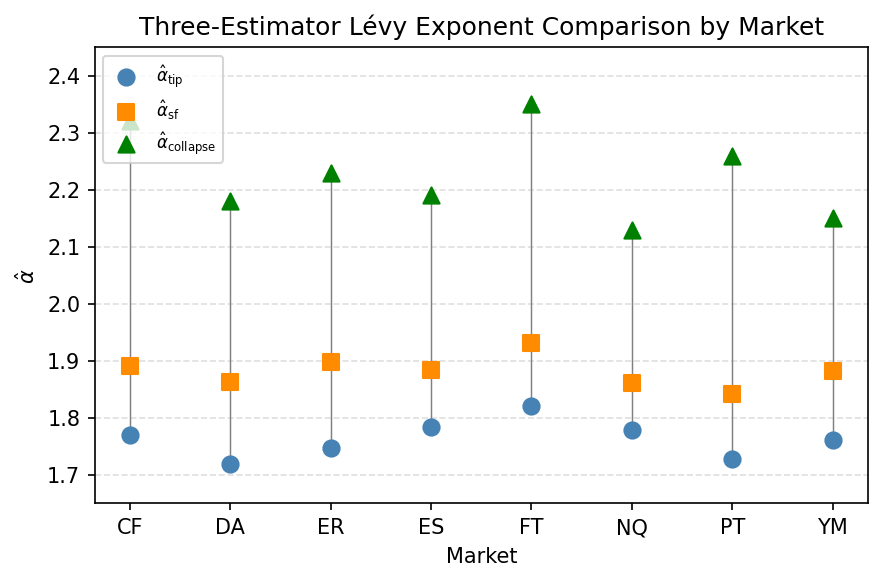
\includegraphics[width=\columnwidth]{figures/fig_three_estimators.png}
\caption{Three-Estimator Scaling Exponent Comparison by Market. Error bars
show the standard deviation of $\alphah$ across the ten
$(\varepsilon,N_\tau)$ design cells; they measure sensitivity to tuning
choices, not sampling uncertainty.}
\label{fig:three_estimators}
\end{figure}

\subsection{Robustness}
\label{sec:results:robustness}

The full factorial robustness matrix enumerates all combinations of resolution
$\varepsilon\in\{0.1,\ldots,0.5\}$, lag grid density $N_\tau\in\{20,37\}$,
preprocessing (raw or deseasonalized), and estimator (tip, sf, collapse),
yielding a comprehensive picture of which design choices drive estimation
uncertainty.

Two findings stand out.
First, within a fixed estimator, $\alphah$ is largely insensitive to
$\varepsilon$ and $N_\tau$. For the two regression-based estimators the
standard deviation of $\alphah$ across the five resolution values and two
grid densities is below $0.032$ for every market (tip) and below $0.002$
(structure functions). The collapse estimator is markedly less stable, with
standard deviations up to $0.107$, reflecting its dependence on the sparsely
populated tails of the rescaled densities.
Second, the estimator choice is the dominant source of variation.
For the same market, preprocessing, $\varepsilon$, and $N_\tau$, the mean
estimated exponents across estimators differ by 0.23--0.36 units, of which
$62\%$ on average separates the collapse criterion from the two
regression-based estimators.
Even the narrower gap between the latter two exceeds the inter-market
spread ($\alphah_{\mathrm{tip}}$ ranges from 1.72 to 1.82 across all eight
markets), which implies that reported $\alphah$ values from different
studies using different estimators cannot be directly compared without
controlling for the estimation principle.

The gap between tip and the other two estimators is also informative about
the mechanism studied in Section~\ref{sec:results:bias}: the tip estimator
is the most sensitive to the central PDF value at each lag, which is where
the short-term mean-reversion bias is concentrated.
This observation motivates the bias correction applied in that section.


\begin{table}[!t]
\begin{center}
\caption{Mean Absolute Asymmetry Ratio by Market}
\begin{tabular}{lc}
\hline
Market & $\bar{A} \equiv \overline{|A(x,\tau)|}_{x>0,\,\tau}$ \\
\hline
NQ & 0.270 \\
DA & 0.297 \\
ER & 0.316 \\
YM & 0.344 \\
ES & 0.397 \\
FT & 0.403 \\
CF & 0.409 \\
PT & 0.463 \\
\hline
\multicolumn{2}{l}{$\varepsilon=0.1$, $N_\tau=20$.}
\end{tabular}
\label{tab:asymmetry}
\end{center}
\end{table}

\subsection{Asymmetry}
\label{sec:results:asymmetry}

The symmetric Lévy model assumes that the positive and negative tails of the
increment distribution have the same shape.
This is tested via the pointwise relative asymmetry ratio
$A(x,\tau) = [\Ph(x,\tau) - \Ph(-x,\tau)]/[\Ph(x,\tau) + \Ph(-x,\tau)]$,
which is zero for a perfectly symmetric distribution and $\pm 1$ at the extremes.
The scalar summary per market is the mean of $|A(x,\tau)|$ over $x>0$,
averaged further over the full lag grid.

Table~\ref{tab:asymmetry} reports these values across markets.
The most symmetric market is NQ (0.27), followed by DA (0.30) and ER (0.32);
the least symmetric is PT (0.46), with CF (0.41) and FT (0.40) also above
the cross-market average of $0.36$.
These aggregate ratios are dominated by the behavior at the very shortest
lags and in the far tails, where histogram estimates are sparse and noisy and
the ratio saturates towards its bound of 1.
Restricting attention to the lag at which each market is most symmetric, the
mean $|A|$ falls to between $0.09$ (NQ) and $0.33$ (PT), and the cross-market
ordering is preserved; the asymmetry is therefore a persistent but moderate
feature rather than an artefact of a single lag.

Symmetrizing the empirical PDF, $\Ph_{\mathrm{sym}}(x,\tau) =
[\Ph(x,\tau)+\Ph(-x,\tau)]/2$, has a substantial and inconsistent effect on
the collapse criterion. At $\varepsilon=0.1$, $N_\tau=20$ it improves the
collapse score in four of the eight markets and worsens it in the other four,
with changes ranging from $-14.5\%$ (ER) to $+50.2\%$ (NQ), and it moves the
minimizing exponent by up to $0.23$ units (CF). The asymmetric component of
the distribution is therefore not negligible for this estimator, which
reinforces the finding of Section~\ref{sec:results:estimators} that the
collapse criterion is the least stable of the three.
There is mild but detectable asymmetry at short lags in several markets,
consistent with bid-ask bounce asymmetry and short-term momentum in futures
order flow; however, its magnitude is small enough that the symmetric Lévy
approximation remains a reasonable first-order description.

\begin{table}[!t]
\begin{center}
\caption{Variance-Ratio Bias Correction by Market}
\begin{tabular}{lccccc}
\hline
Market & $\rhoh(1)$ & $\VRh_{60}$ & $\alphah_{\mathrm{tip}}$
       & $\alphah_{\mathrm{corr}}$ & $\widehat{\Delta\alpha}$ \\
\hline
PT & $-0.020$ & 0.895 & 1.709 & 1.695 & $+0.014$ \\
DA & $-0.008$ & 0.949 & 1.709 & 1.703 & $+0.006$ \\
ES & $-0.008$ & 0.949 & 1.791 & 1.785 & $+0.006$ \\
YM & $-0.004$ & 0.951 & 1.755 & 1.748 & $+0.007$ \\
FT & $-0.009$ & 0.952 & 1.809 & 1.802 & $+0.007$ \\
ER & $+0.001$ & 0.958 & 1.725 & 1.718 & $+0.007$ \\
CF & $-0.007$ & 0.974 & 1.752 & 1.749 & $+0.003$ \\
NQ & $-0.001$ & 0.980 & 1.746 & 1.743 & $+0.003$ \\
\hline
\multicolumn{6}{l}{$\varepsilon=0.1$, $N_\tau=20$, $K_{\max}=60$; sorted by $\VRh_{60}\uparrow$.}
\end{tabular}
\label{tab:bias}
\end{center}
\end{table}

\subsection{Bias correction}
\label{sec:results:bias}

Step~6 of Algorithm~\ref{alg:pipeline} implements the bias correction
described in Section~\ref{sec:methodology:bias}.
Seven of the eight markets exhibit negative first-order autocorrelation of
1-minute returns; ER displays a statistically negligible first-order autocorrelation
($\rhoh(1)=+0.001\approx 0$), but its 60-lag cumulative variance ratio $\VRh_{60}=0.958<1$
confirms it is also mean reverting at longer horizons.
Table~\ref{tab:bias} reports the estimated first-order autocorrelation
$\rhoh(1)$, the 60-lag cumulative variance ratio
$\VRh_{60} = 1 + 2\sum_{k=1}^{K_{\max}}\rhoh(k)$, the uncorrected tip estimate
$\alphah_{\mathrm{tip}}$, the bias-corrected estimate $\alphah_{\mathrm{corr}}$,
and the implied correction $\widehat{\Delta\alpha} = \alphah_{\mathrm{tip}}
- \alphah_{\mathrm{corr}}$.
For reference the table is sorted by $\VRh_{60}$ in ascending order (strongest
mean reversion first).

The bias correction reduces $\alphah_{\mathrm{tip}}$ for all eight markets, and the markets with
the smallest $\VRh_{60}$ (strongest net mean reversion) display the largest
corrections.
PT, which has $\VRh_{60} = 0.895$ and $\rhoh(1) = -0.020$, is the most
mean-reverting contract and shows the largest downward correction
($\widehat{\Delta\alpha}\approx 0.014$).
The corrections are uniformly small: at most $0.014$ units, against a
dispersion of up to $0.032$ induced in $\alphah_{\mathrm{tip}}$ by varying
$\varepsilon$ and $N_\tau$ alone (Section~\ref{sec:results:robustness}).
The adjustment is therefore systematic in sign and ordering but smaller than
the estimator's own sensitivity to design choices, so it should be read as
below the practical resolution of the method on this sample rather than as
evidence that discreteness-driven bias is absent.
Although ER has a marginally positive first-order autocorrelation
($\rhoh(1) = +0.001$), its 60-lag cumulative variance ratio $\VRh_{60} = 0.958$
remains below 1, indicating that negative autocorrelations at longer lags
dominate; the correction is therefore downward, with magnitude
$\widehat{\Delta\alpha} = 0.007$.
Across the cross section $\widehat{\Delta\alpha}$ decreases with
$\VRh_{60}$, with a Pearson correlation of $-0.98$ between the two
quantities: the markets furthest from the martingale benchmark receive the
largest corrections, and those closest to it the smallest. The linear
association is dominated by PT, the most strongly mean-reverting contract;
the rank correlation is a weaker $-0.62$, and the ordering is
not strictly monotone at the market level, as the five contracts with
$\VRh_{60}$ between $0.949$ and $0.958$ are separated by less than
$0.01$ in variance ratio and their corrections differ by under
$0.002$ exponent units, which is within the estimation noise of
$\widehat{\Delta\alpha}$. The systematic negative association is nonetheless
consistent with the bias mechanism derived in
Section~\ref{sec:background:vr}.

In further unreported checks, excluding the three shortest lags
($\tau\in\{1,2,3\}$) leaves the ordering unchanged and produces comparable
correction magnitudes, consistent with microstructure effects at very short
horizons being modest; this check bears on discreteness and bounce, not on the
session-index construction discussed in Section~\ref{sec:data:preprocessing}.
A $K_{\max}$ sensitivity analysis on the pilot market (ES) over
$K_{\max}\in\{30,60,120,240\}$ leaves $\alphah_{\mathrm{corr}}$ stable,
well below the inter-estimator spread documented in Section~\ref{sec:results:estimators}.

% ── Bias correction figure ─────────────────────────────────────────────────
\begin{figure*}[!t]
\centering
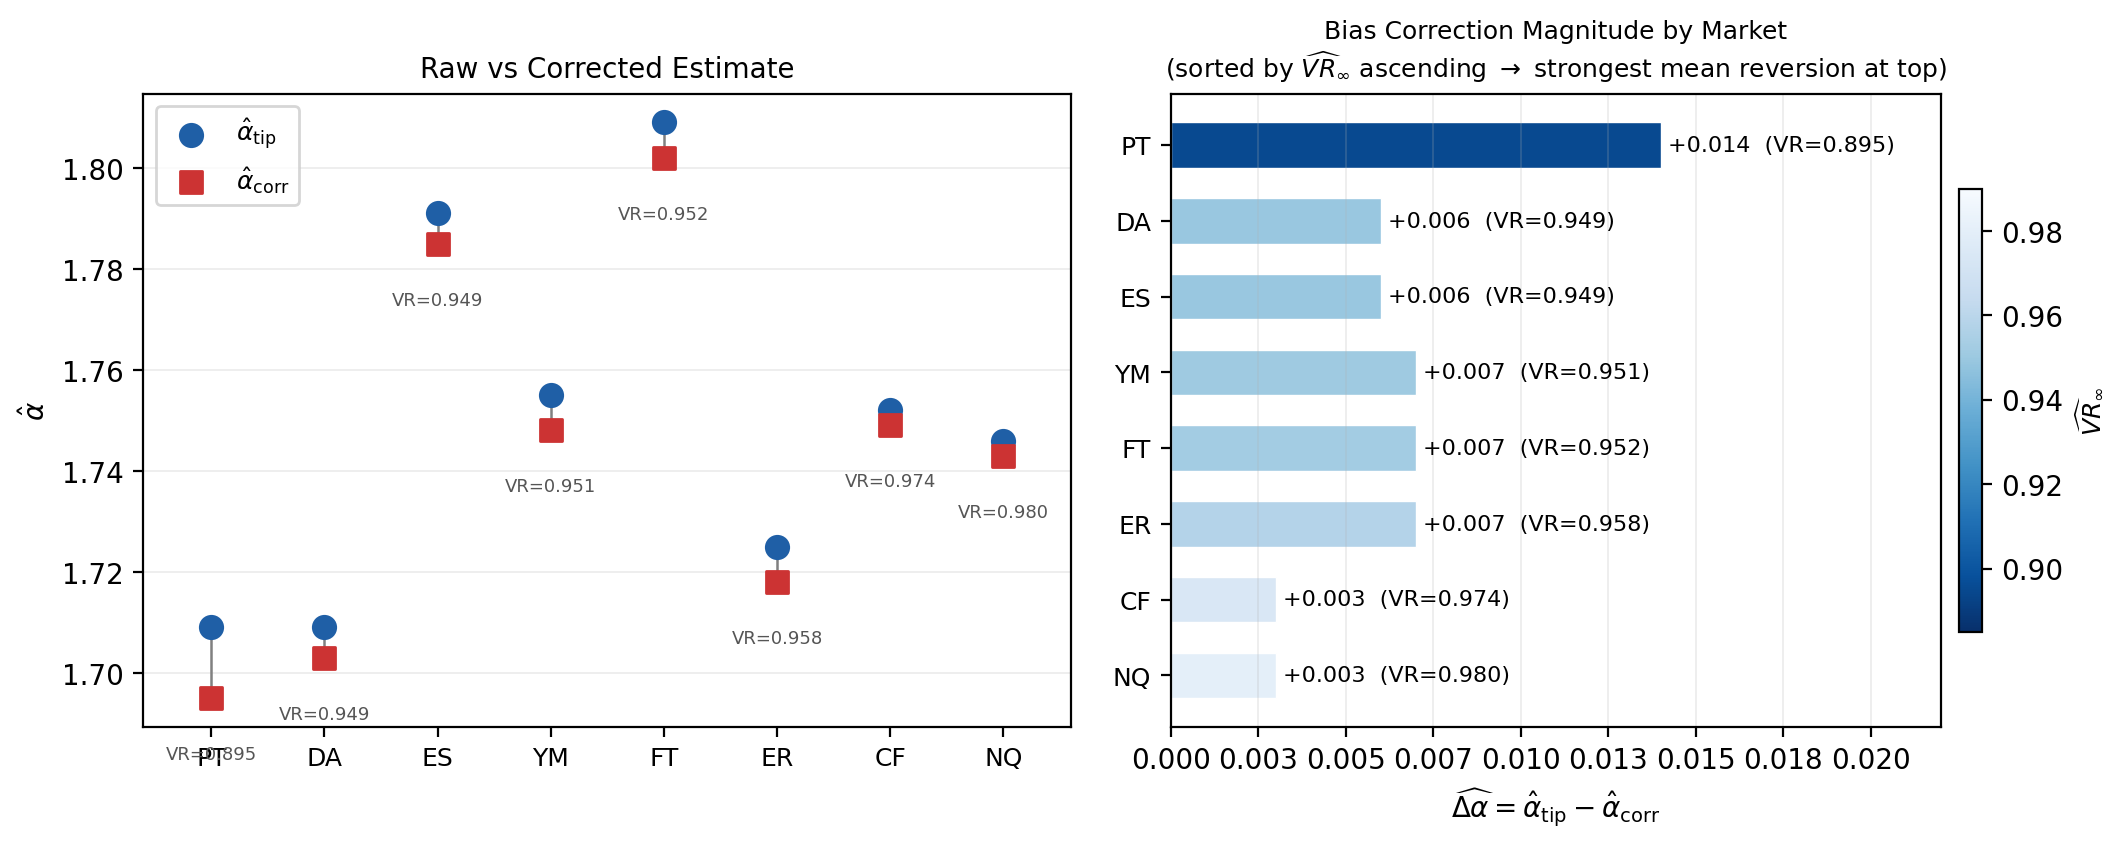
\includegraphics[width=0.92\textwidth]{figures/fig_bias_correction.png}
\caption{Variance-Ratio Bias Correction by Market.}
\label{fig:bias_correction}
\end{figure*}

% ══════════════════════════════════════════════════════════════════════════════
\section{Conclusion}
\label{sec:conclusion}
% ══════════════════════════════════════════════════════════════════════════════

\subsection{Summary of Findings}

This paper has examined Lévy scaling in short-horizon futures returns across
eight equity-index contracts spanning North America and Europe, using
1-minute OHLCV data from the start of available data through January 2026.
Six findings emerge.

\textbf{(i) Baseline scaling.}
All eight markets yield peak scaling exponents lying within
$\alphah_{\mathrm{tip}}\in[1.718,\,1.821]$, with $R^2\geq0.997$ for the log-log
regression in every case.
The cross-market mean is $\bar\alpha\approx 1.76$, consistent with the
Mantegna--Stanley consensus and with prior estimates for equity-index
instruments.
The result holds uniformly across contract specifications that differ by an
order of magnitude in tick size and by a factor of thirteen in $\sigma_1$,
indicating that tick-relative histogram calibration renders the exponent
estimates comparable across markets of very different absolute price scale.

\textbf{(ii) Intraday seasonality.}
Removing the U-shaped intraday volatility profile shifts $\alphah_{\mathrm{tip}}$
upward by $0.027$--$0.095$ exponent units and has a negligible effect on regression
quality ($|\Delta R^2|<0.003$).
The shift is uniformly positive across all eight markets.
Intraday seasonality is therefore not a dominant confound for Lévy scaling
estimation at the 1-minute frequency.

\textbf{(iii) Estimator comparison.}
Of the three distinct estimators applied (tip scaling OLS, collapse quality
minimization, and fractional order structure functions), the two
regression-based methods are broadly consistent, differing by $0.083$--$0.152$
units, whereas the collapse criterion sits a further $0.145$--$0.248$ units
higher and exceeds the stable-law boundary in every market.
The systematic ordering $\alphah_{\mathrm{tip}}<\alphah_{\mathrm{sf}}<
\tilde{\alpha}_{\mathrm{collapse}}$ holds for all eight markets, with
inter-estimator spreads of $0.23$--$0.36$ units.
This gap is substantially larger than the inter-market spread, implying that
reported $\alphah$ values from different studies cannot be directly compared
without controlling for the estimation principle.

\textbf{(iv) Robustness.}
Within the two regression-based estimators, $\alphah$ is largely insensitive
to histogram resolution $\varepsilon$ and lag grid density $N_\tau$: the
standard deviation across these design choices stays below $0.032$ for the
peak scaling estimator and below $0.002$ for the structure functions, against
up to $0.107$ for the collapse estimator.
The estimator choice, not the tuning parameters, is the dominant source of
variation in reported $\alphah$ values.

\textbf{(v) Symmetry.}
The empirical PDFs exhibit mild but detectable asymmetry,
with mean absolute asymmetry ratios ranging from $0.27$ (NQ) to $0.46$ (PT)
in aggregate.
At the lag where each market is most symmetric the ratio falls to between
$0.09$ (NQ) and $0.33$ (PT), so the asymmetry is moderate but persistent
across the lag grid rather than confined to the shortest lags.
Symmetrizing the PDFs before collapse matching changes the collapse score by
$-14.5\%$ to $+50.2\%$ across markets and shifts the minimizing exponent by up
to $0.23$ units, so the symmetric approximation is adequate for the two
regression-based estimators but not for the collapse criterion.

\textbf{(vi) Bias correction.}
Seven of the eight markets exhibit negative first-order autocorrelation; ER
displays a statistically negligible $\rhoh(1)=+0.001\approx 0$ but is
mean reverting over the 60-lag window ($\VRh_{60}=0.958<1$) and therefore
corrects downward like the rest.
The 60-lag cumulative variance ratios span $\VRh_{60}\in[0.895,\,0.980]$.
For all eight markets the variance-ratio correction reduces
$\alphah_{\mathrm{tip}}$ by $\widehat{\Delta\alpha}\in[0.003,\,0.014]$, and
the correction magnitude is strongly negatively associated with
$\VRh_{60}$ (Pearson $-0.98$ across eight markets, from which no significance
is claimed). Since $b(\tau)$ and $\VRh_{60}$ are both
functions of the same estimated autocorrelations, this association is largely
mechanical and is reported as a cross-sectional consistency check rather than
as independent validation of the bias mechanism.
The corrected estimates fall within the interval $[1.695,\,1.802]$,
consistent with historical Lévy-finance benchmarks.

\subsection{Limitations}
Several caveats apply.
The study covers a single asset class; whether the $\alpha\approx 1.7$--$1.8$
finding extends to foreign exchange, commodity, or fixed-income futures is an
open question.
The peak scaling estimator targets the body of the distribution rather than
the tail index in the Hill--Pickands sense, and the two need not coincide for
truncated Lévy flights.
The bias correction is derived under covariance-stationarity; at the very
shortest lags, microstructure effects such as bid-ask bounce and price
discreteness can introduce deviations that the correction does not fully absorb.
Sampling uncertainty is not quantified: every dispersion reported here is
variation across design choices, and no standard errors or confidence
intervals are attached to $\alphah$. Constructing them is awkward on this
grid, since the longest lag spans roughly $139$ trading days and any block
resampling scheme must use blocks far longer than that.
Two properties of the underlying series also warrant caution. First, the
increments are unnormalized changes in index points, so a fixed move carries a
different proportional meaning at the start and end of samples spanning two to
three decades of index growth; the pooled distribution is therefore not
strictly stationary. Second, the roll convention of the vendor's continuous
series is not disclosed, so increments spanning a contract transition cannot be
identified and excluded.

\subsection{Extensions}
Longer samples would allow the temporal stability of $\alphah$ to be assessed
and would permit the cross-market correlation of exponent estimates to be
studied as a possible systemic risk indicator.
Applying the same framework to GARCH-filtered residuals would separate the
contribution of conditional heteroscedasticity from the unconditional tail
behavior.
Finally, extending the lag grid to sub-minute frequencies, where Lévy
scaling is expected to break down due to price-grid discreteness, would
sharpen the lower boundary of the self-similar regime.


% ══════════════════════════════════════════════════════════════════════════════
\section*{Author Contributions}
All authors contributed equally, and their names are listed in alphabetical order.

\bibliographystyle{IEEEtran}
\bibliography{references}

\end{document}
